\section{Results}

\subsection{Calculation of the Monthly mean of Chlorophyll-a Concentration in the East Sea (Sea of Japan)}


The result of monthly-mean chlorophyll-a concentration using the GAC data and the LAC data from 2003 to 2006 is shown in Figure \ref{fig:monLAC01}. - Figure \ref{fig:monLAC03}. The monthly-mean chlorophyll-a concentration of GAC data from 2003 to 2006 is shown in Figure \ref{fig:monGAC01} - Figure \ref{fig:monGAC03}. In these figures, the grey area is land of western part of Korean and southeastern part of Japan. Red area refers to relatively higher concentration compared to the blue area as it is shown at the color bar. Spring (March, April, May) and fall (October, November) show high concentration. 

The black area is part with no data due to cloud coverage or satellite failures. LAC data in 2005 especially show large black ar eas because less files had been aggeragated compared to other years. The black areas in Winter (January, December) can also been noticed to be larger than other years and this is caused by cloud coverage.

\begin{figure}[h]
	\centering
	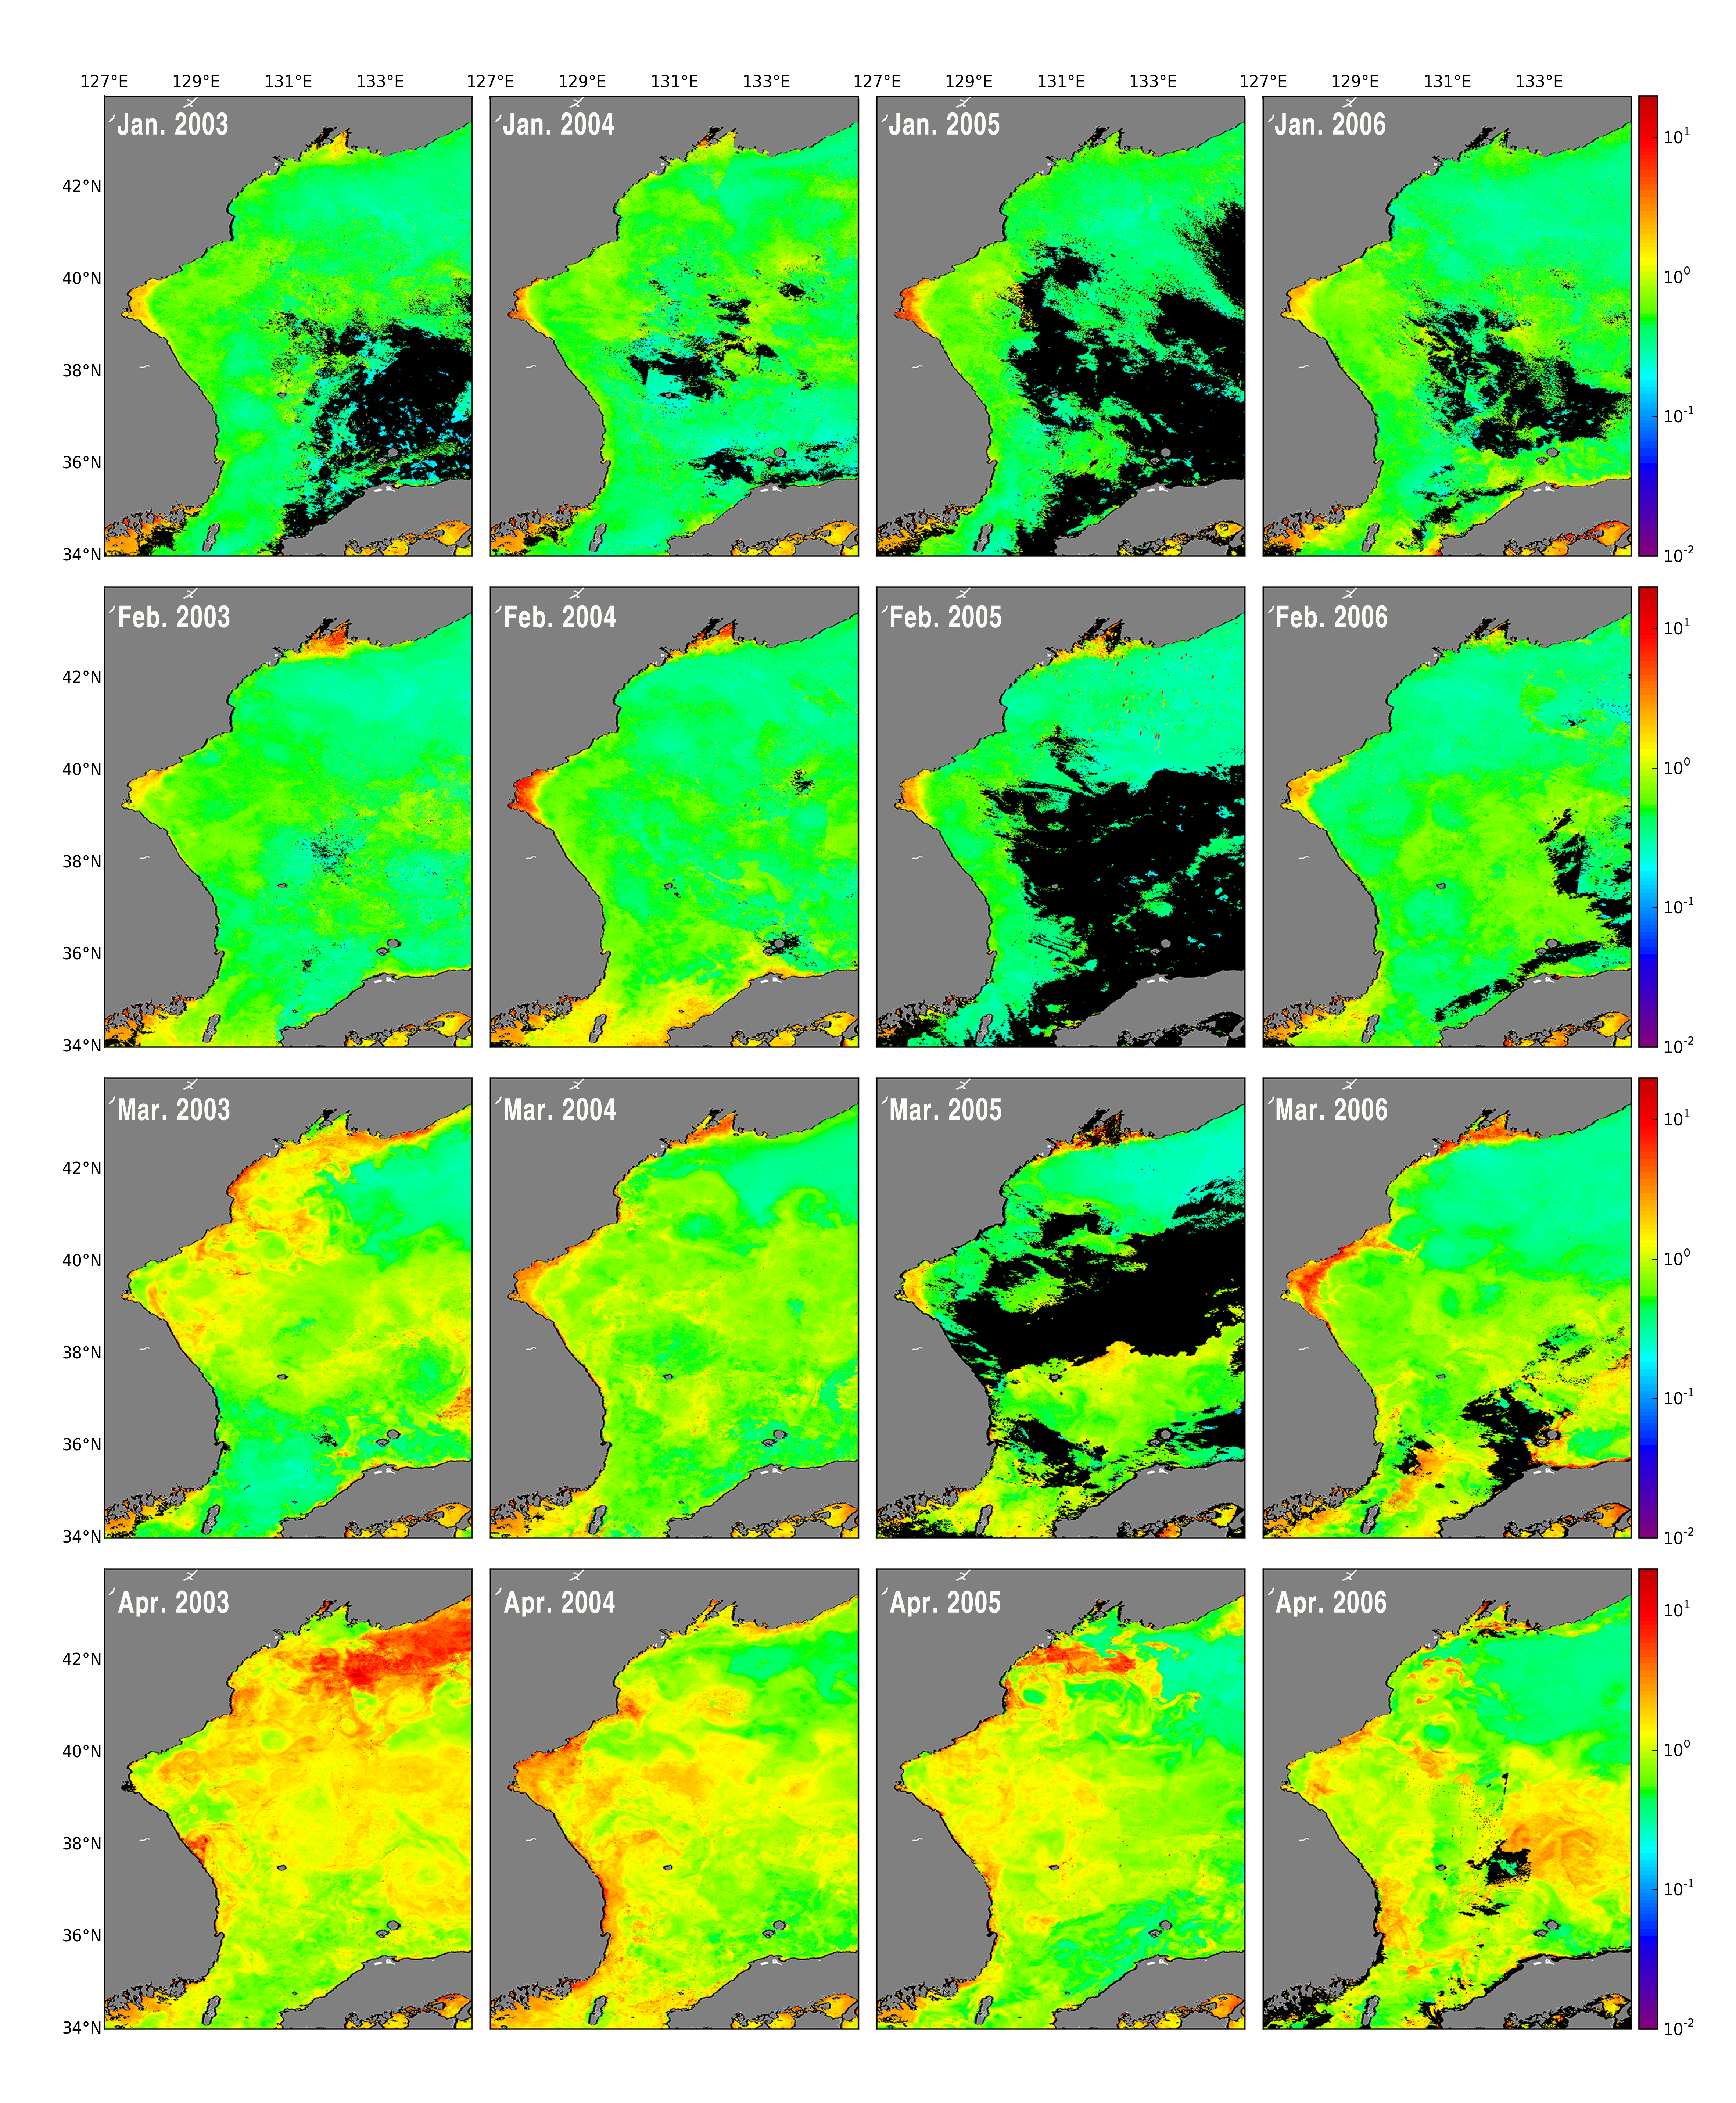
\includegraphics[width=1.0\textwidth]{monLAC01}\\
	\scriptsize\caption{The monthly-mean chlorophyll-a distribution in the East Sea (Sea of Japan), LAC. From 2003 to 2006, January to April. The unit of the color bar is $\rm mg/m^3$.}
	\label{fig:monLAC01}
\end{figure}


\begin{figure}[h]
	\centering
	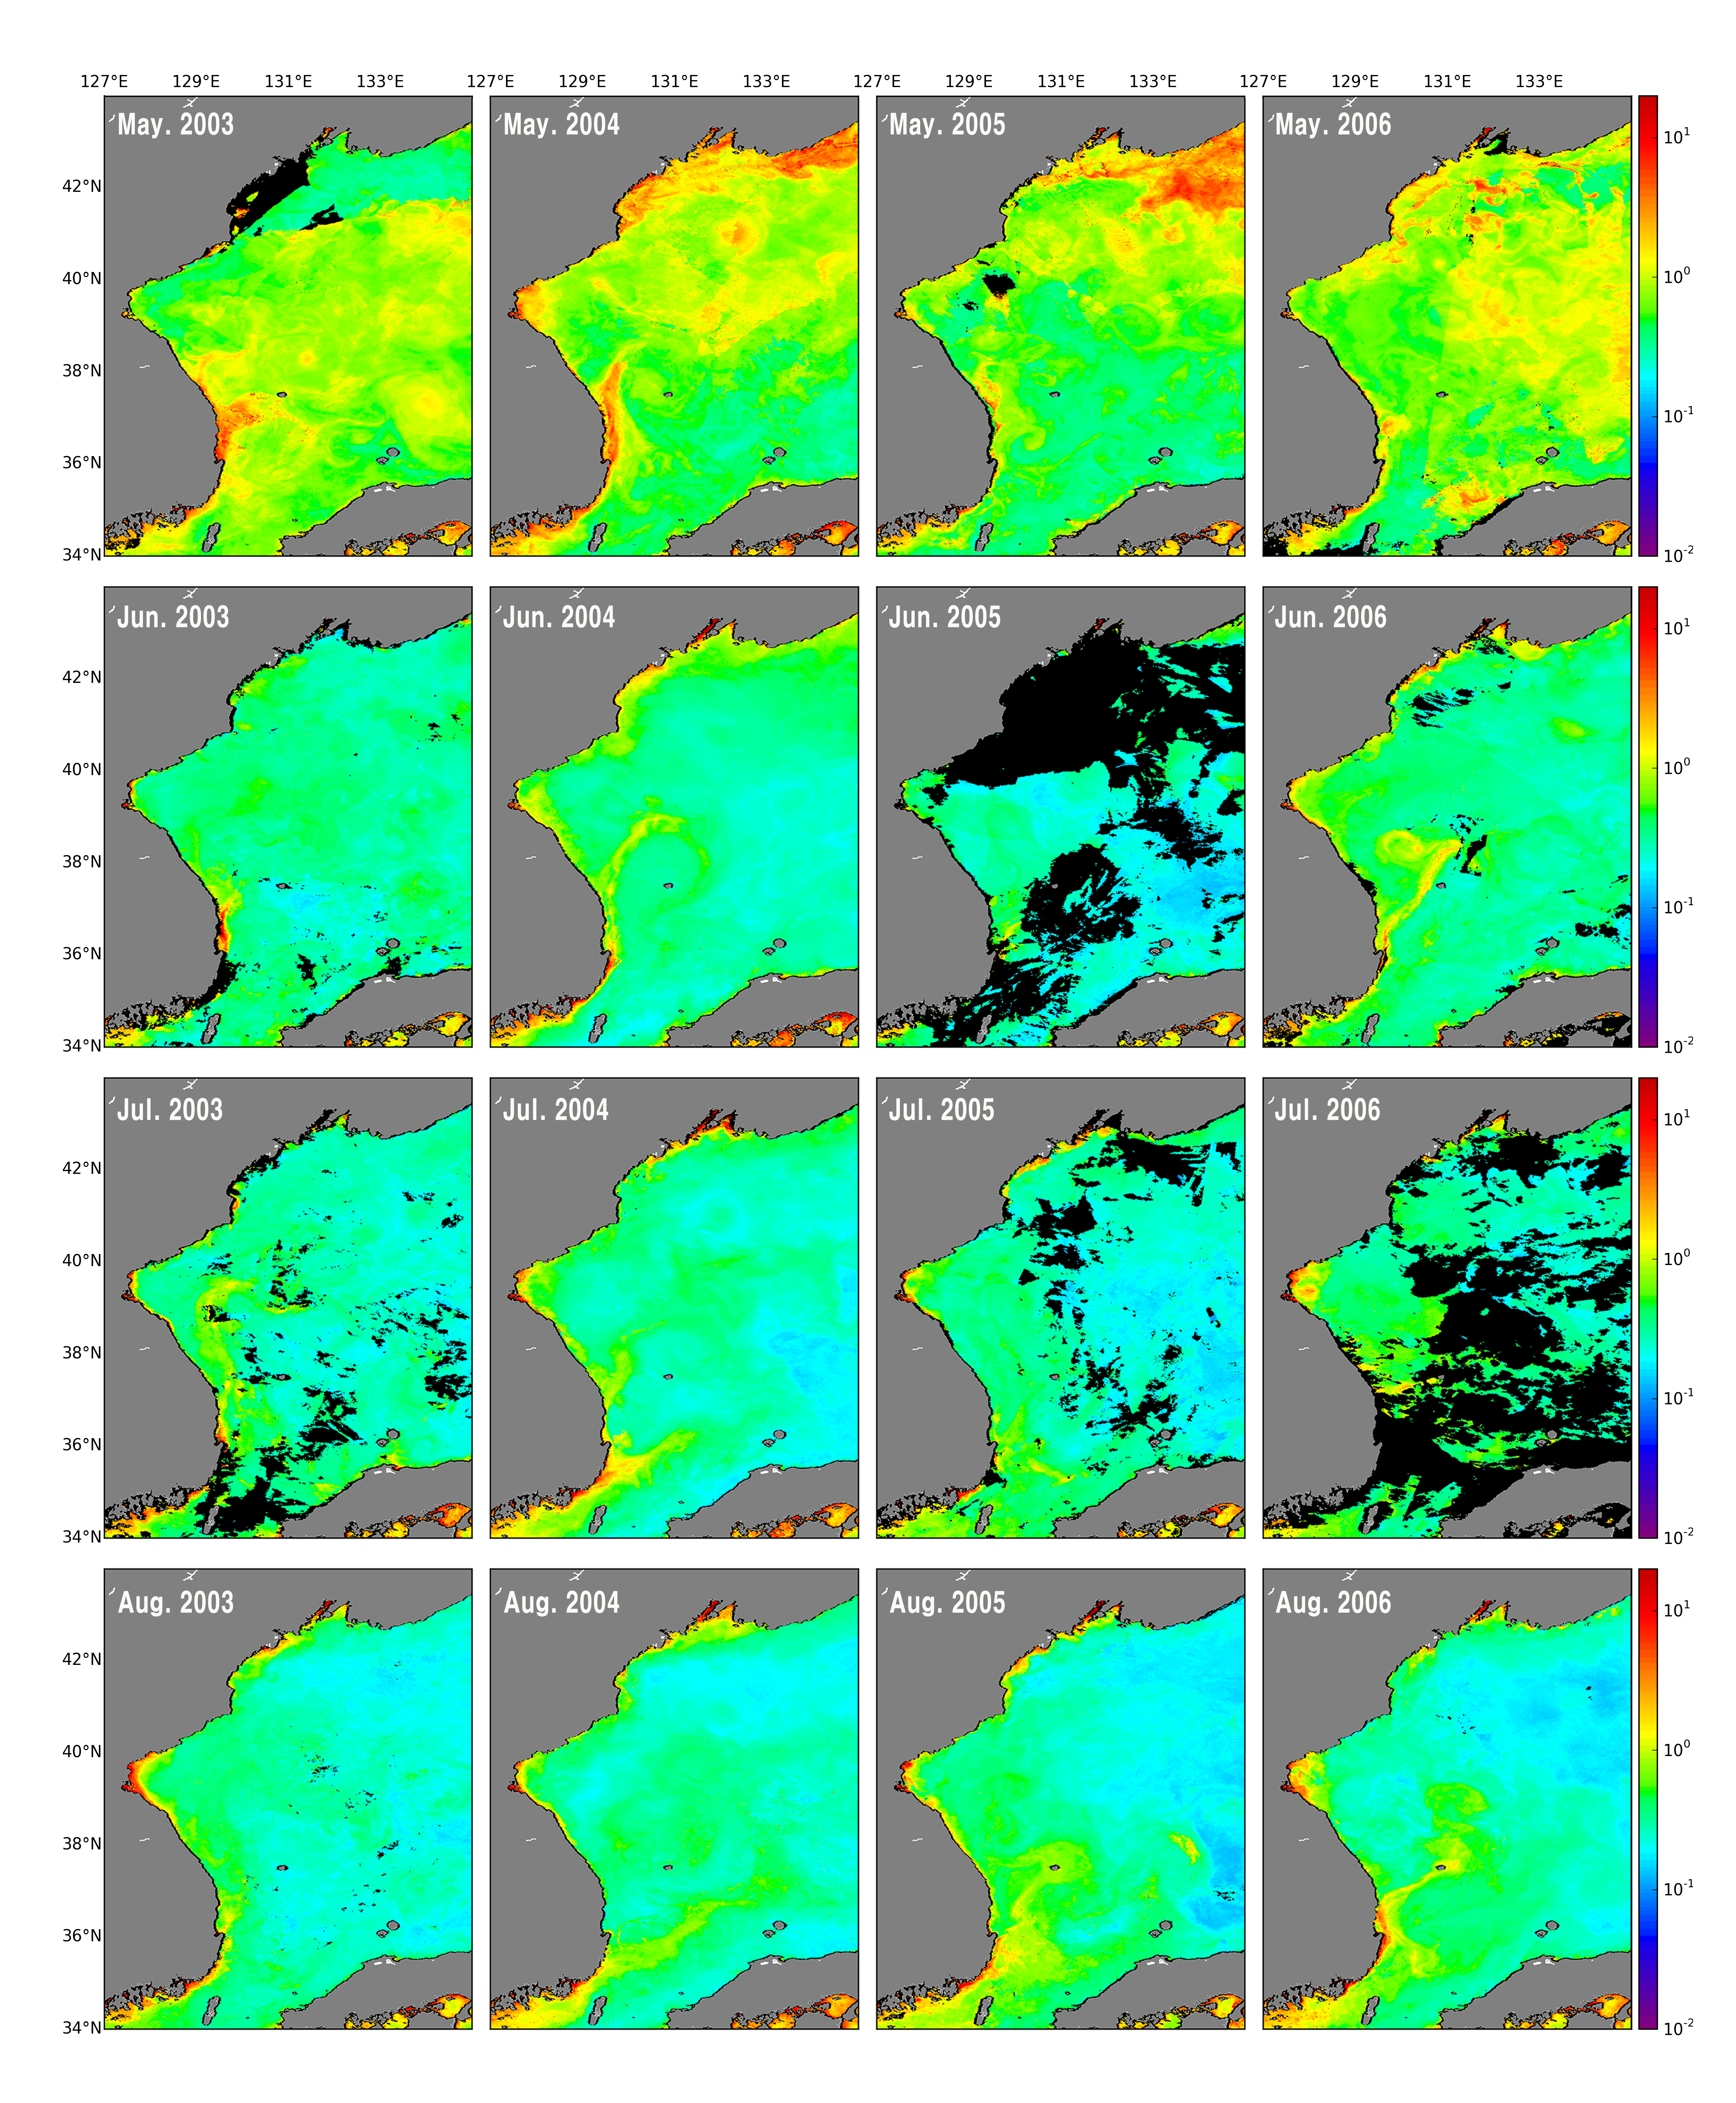
\includegraphics[width=1.00\textwidth]{../images/monLAC02}\\
	\scriptsize\caption{The monthly-mean chlorophyll-a distribution in the East Sea (Sea of Japan), LAC. From 2003 to 2006, May to August. The unit of the color bar is $\rm mg/m^3$.}
	\label{fig:monLAC02}
\end{figure}

\begin{figure}[h]
	\centering
	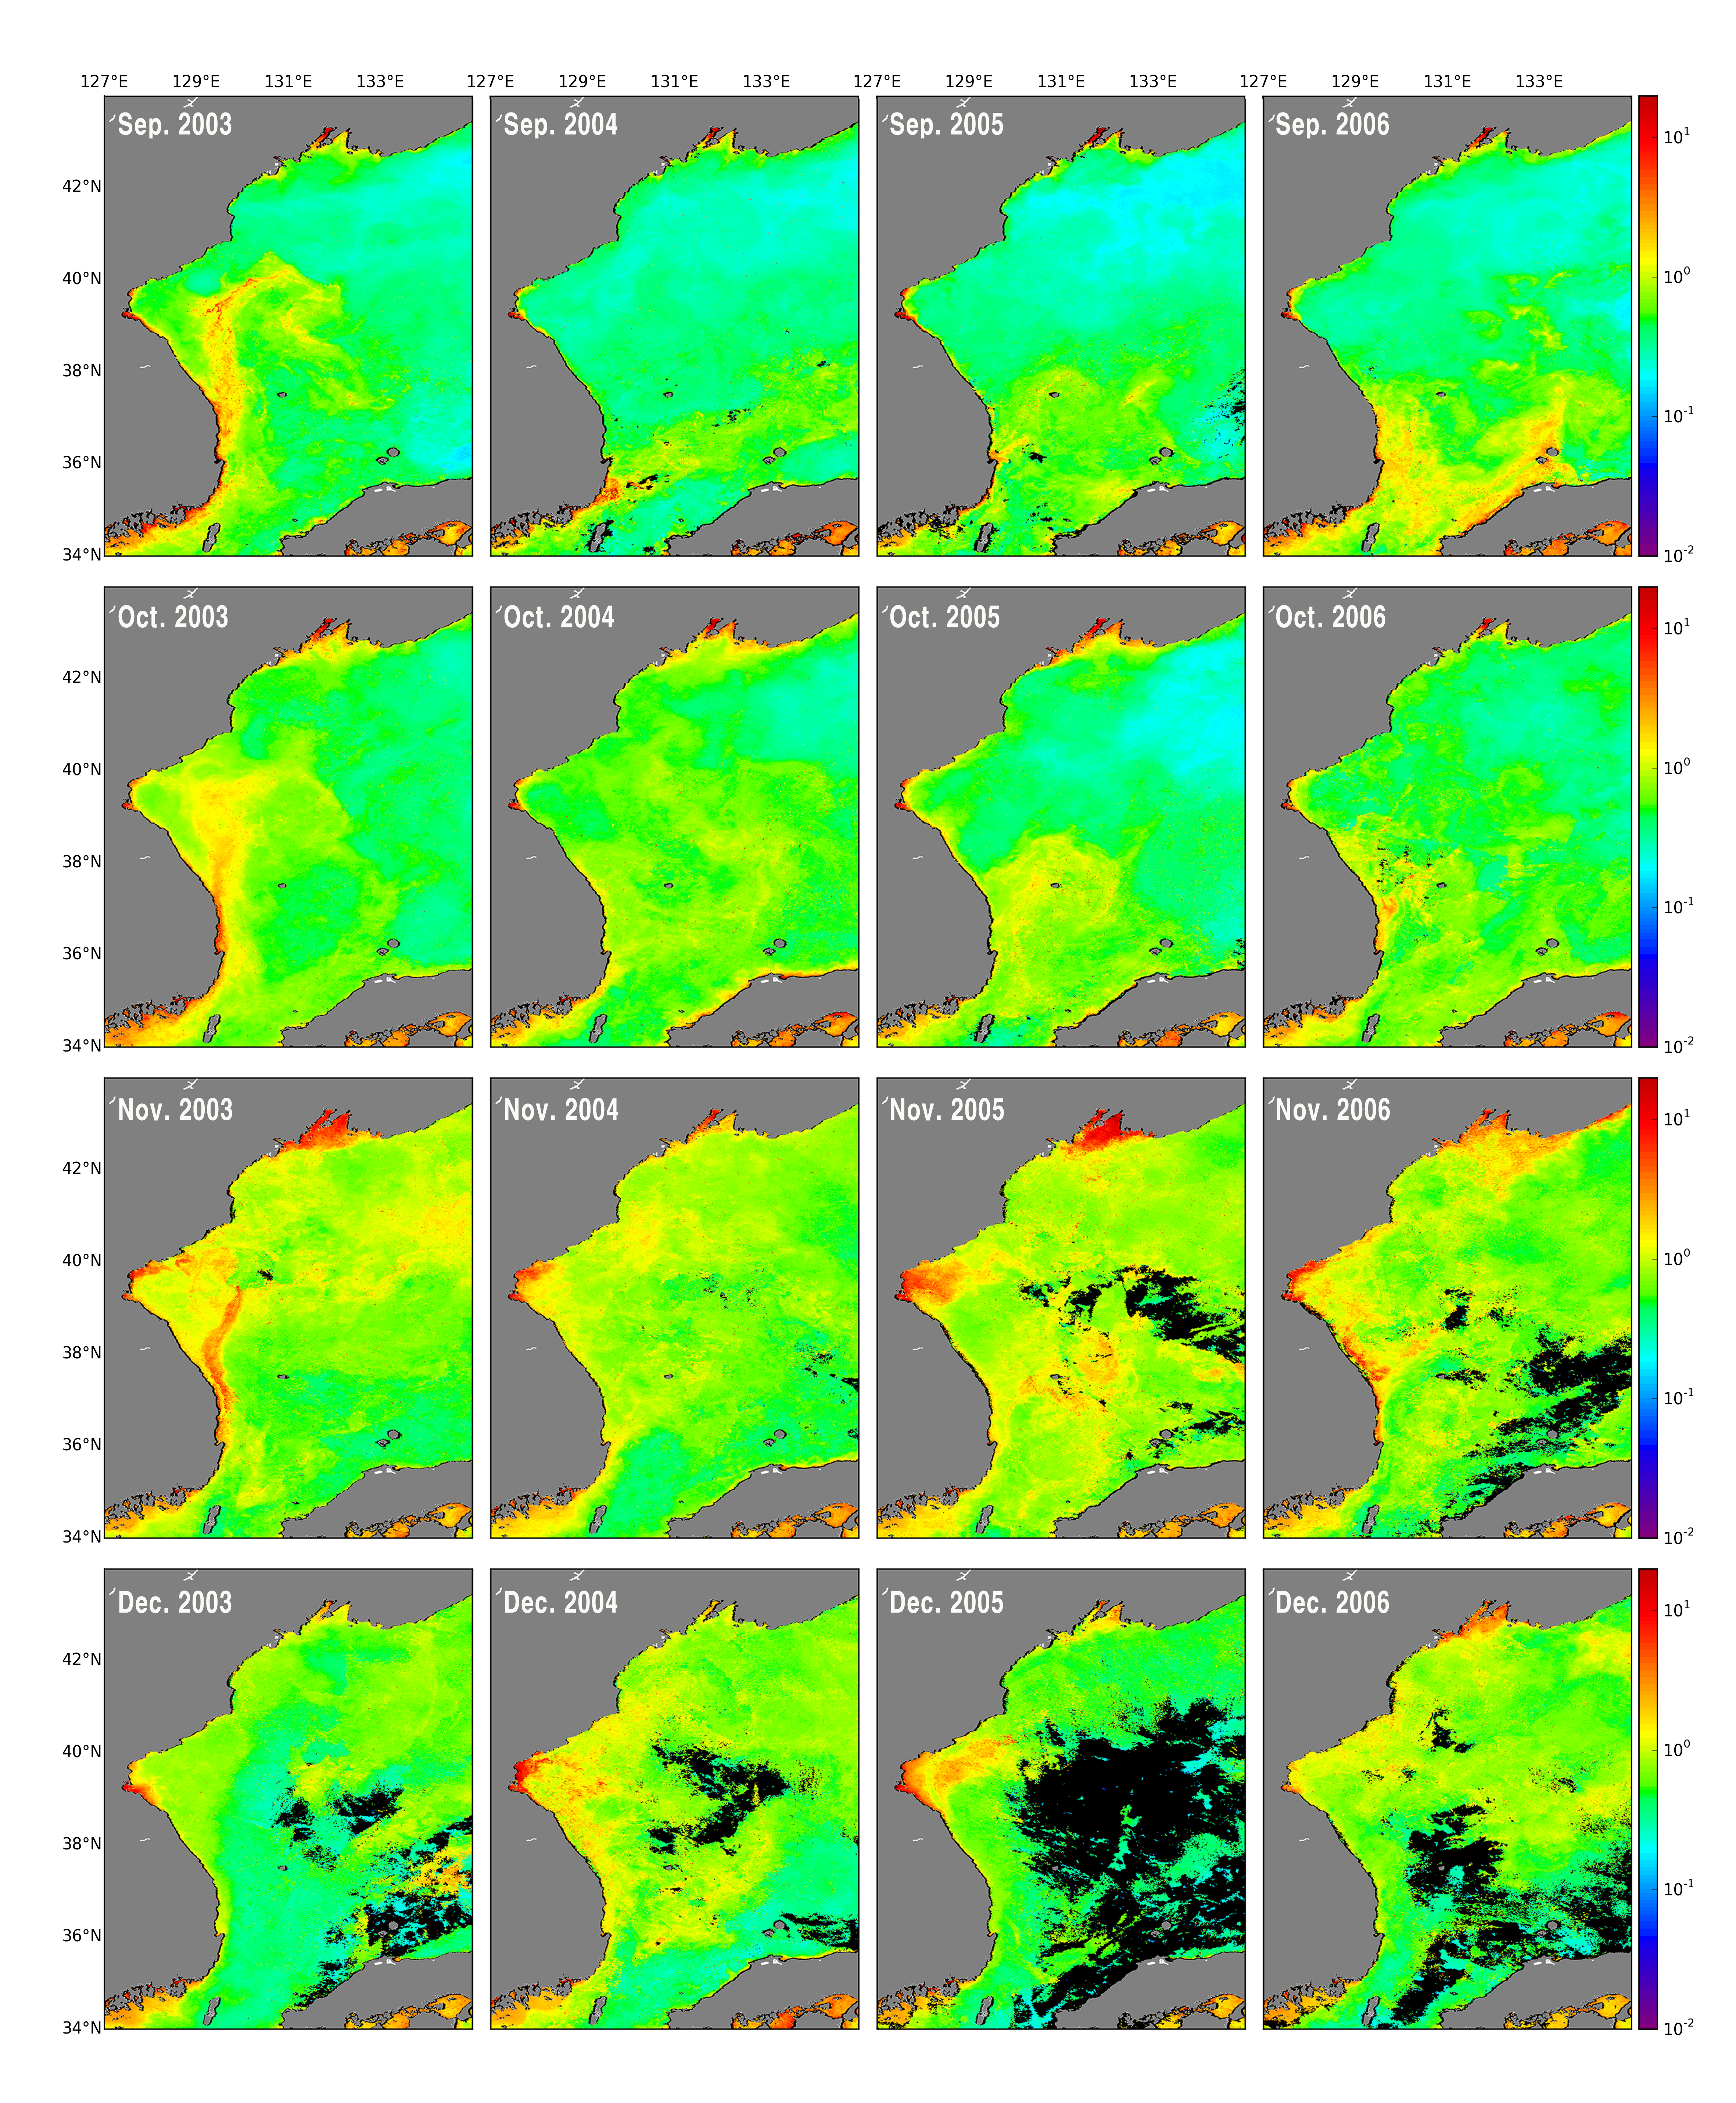
\includegraphics[width=1.00\textwidth]{../images/monLAC03}\\
	\scriptsize\caption{The monthly-mean chlorophyll-a distribution in the East Sea (Sea of Japan), LAC. From 2003 to 2006, September to December. The unit of the color bar is $\rm mg/m^3$.}
	\label{fig:monLAC03}
\end{figure}


\begin{figure}[h]
	\centering
	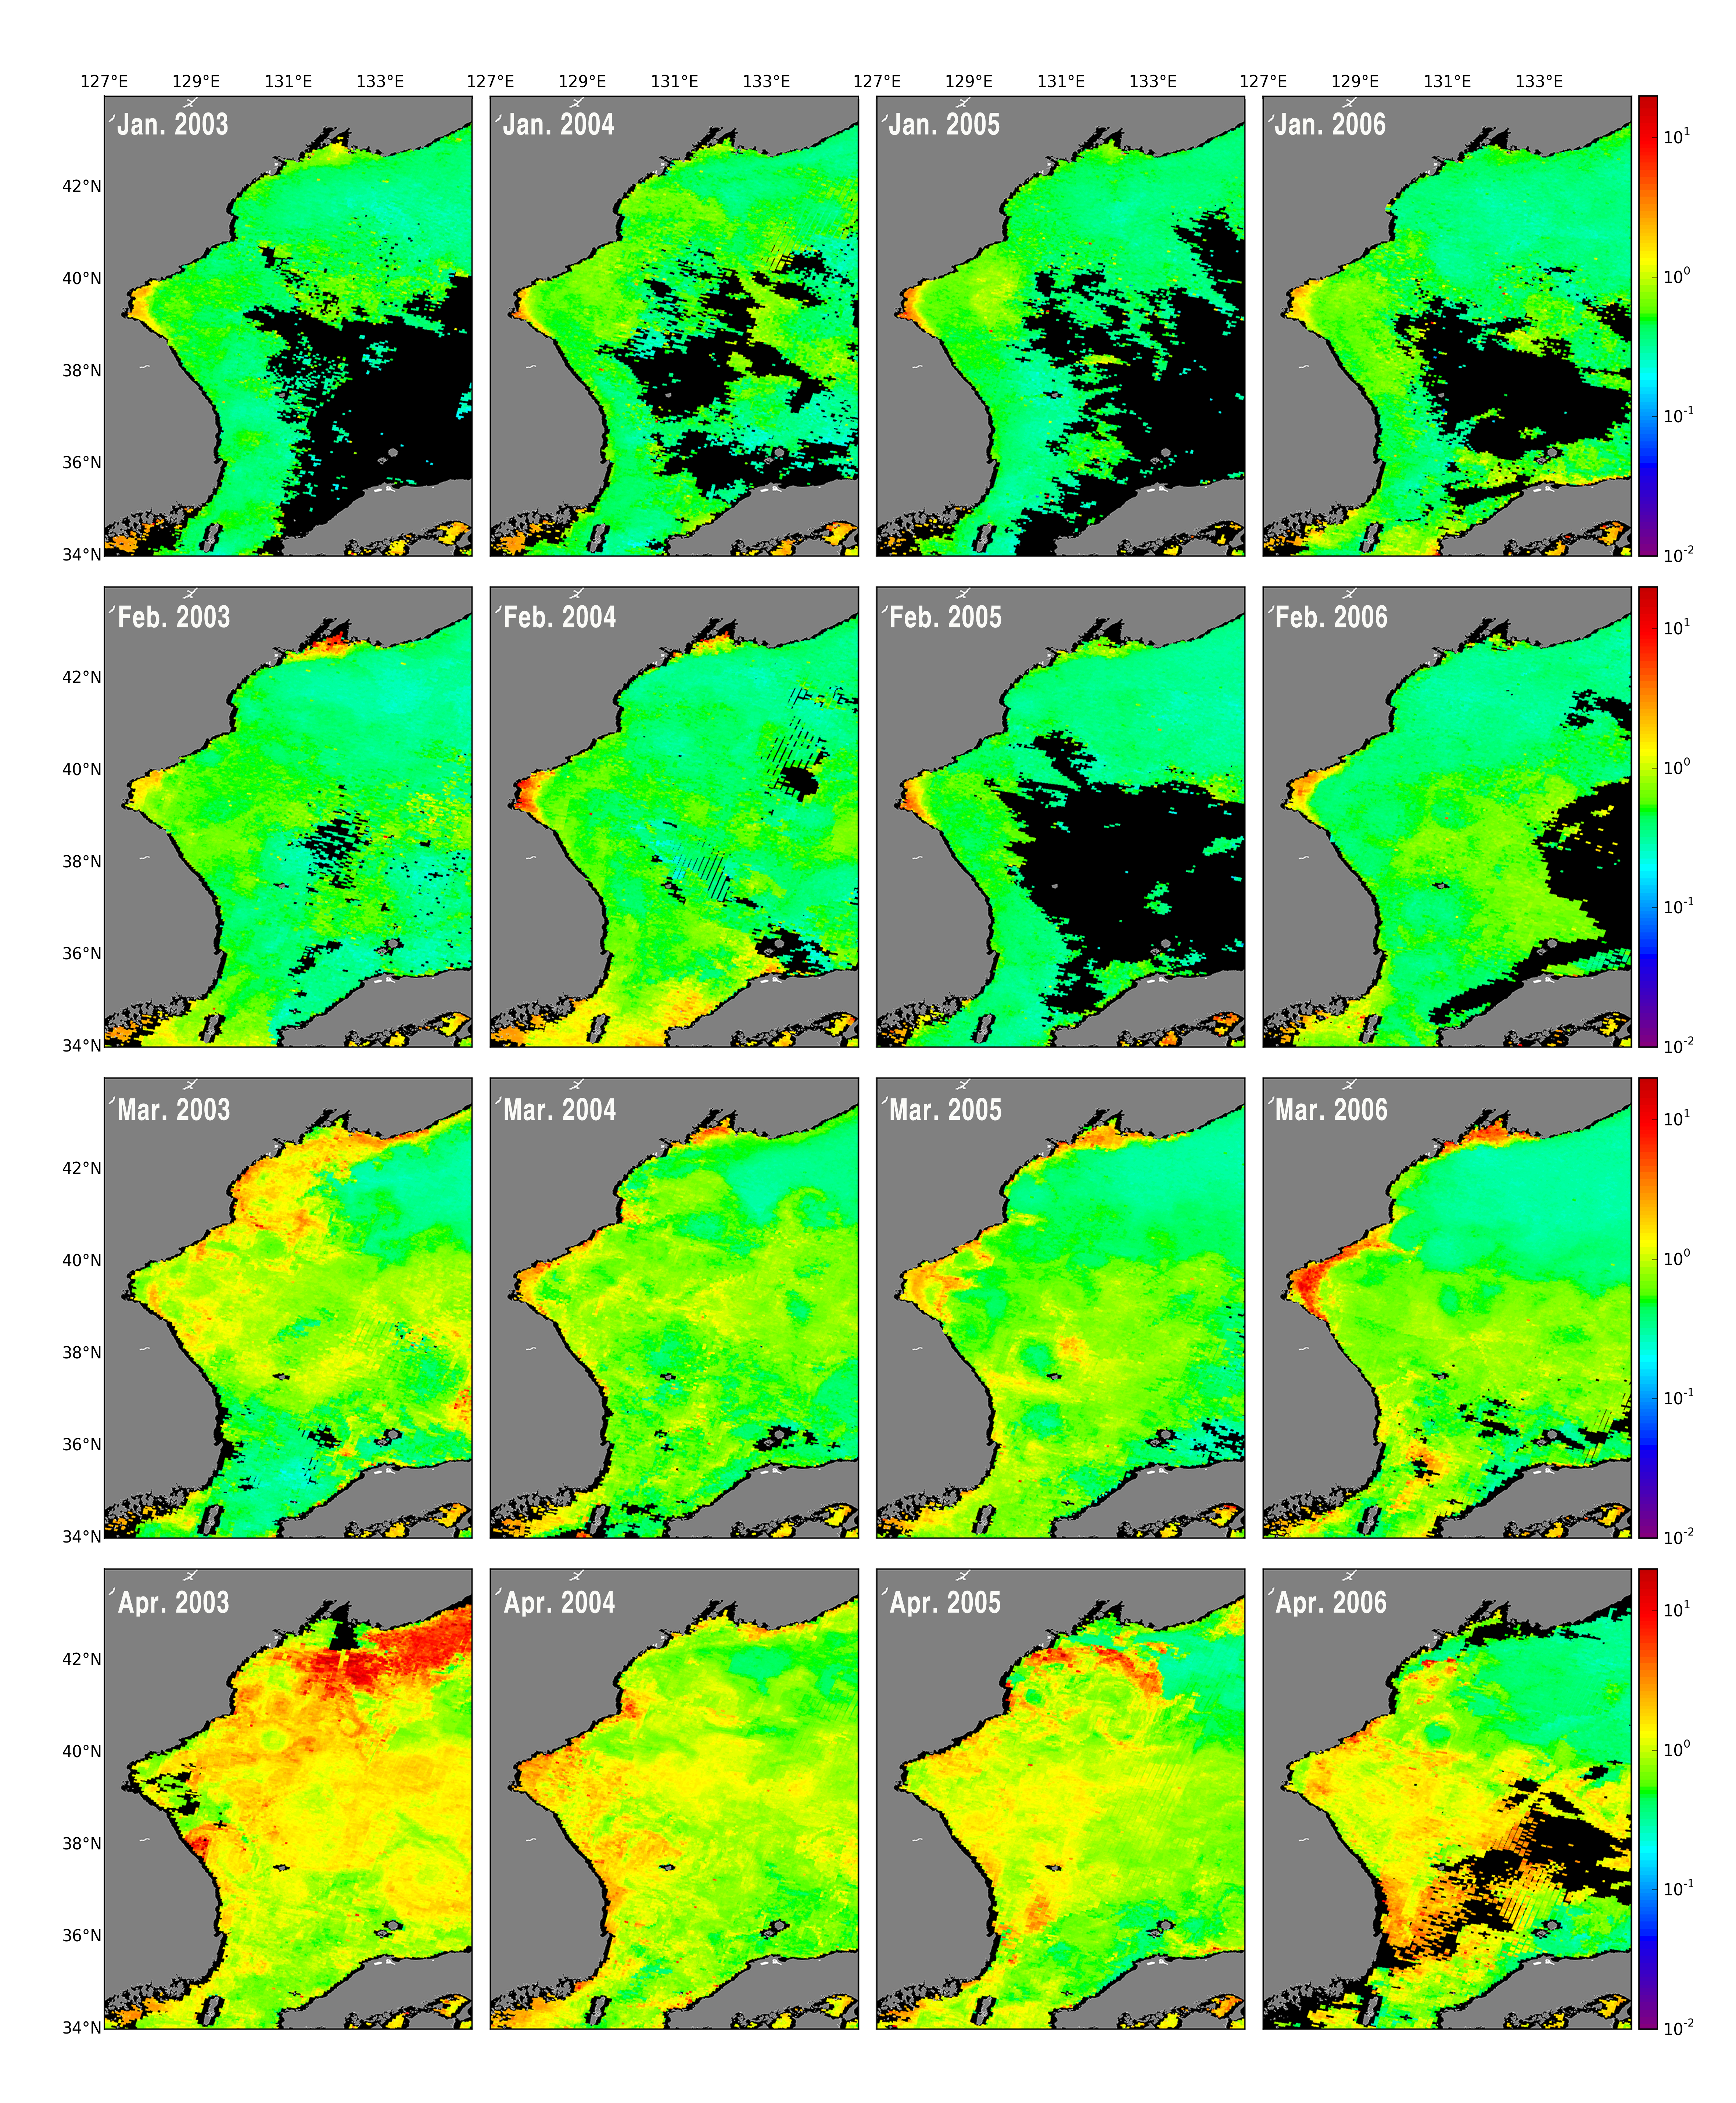
\includegraphics[width=1.0\textwidth]{../images/monGAC01}\\
	\scriptsize\caption{The monthly-mean chlorophyll-a distribution in the East Sea (Sea of Japan), LAC. From 2003 to 2006, January to April. The unit of the color bar is $\rm mg/m^3$.}
	\label{fig:monGAC01}
\end{figure}


\begin{figure}[h]
	\centering
	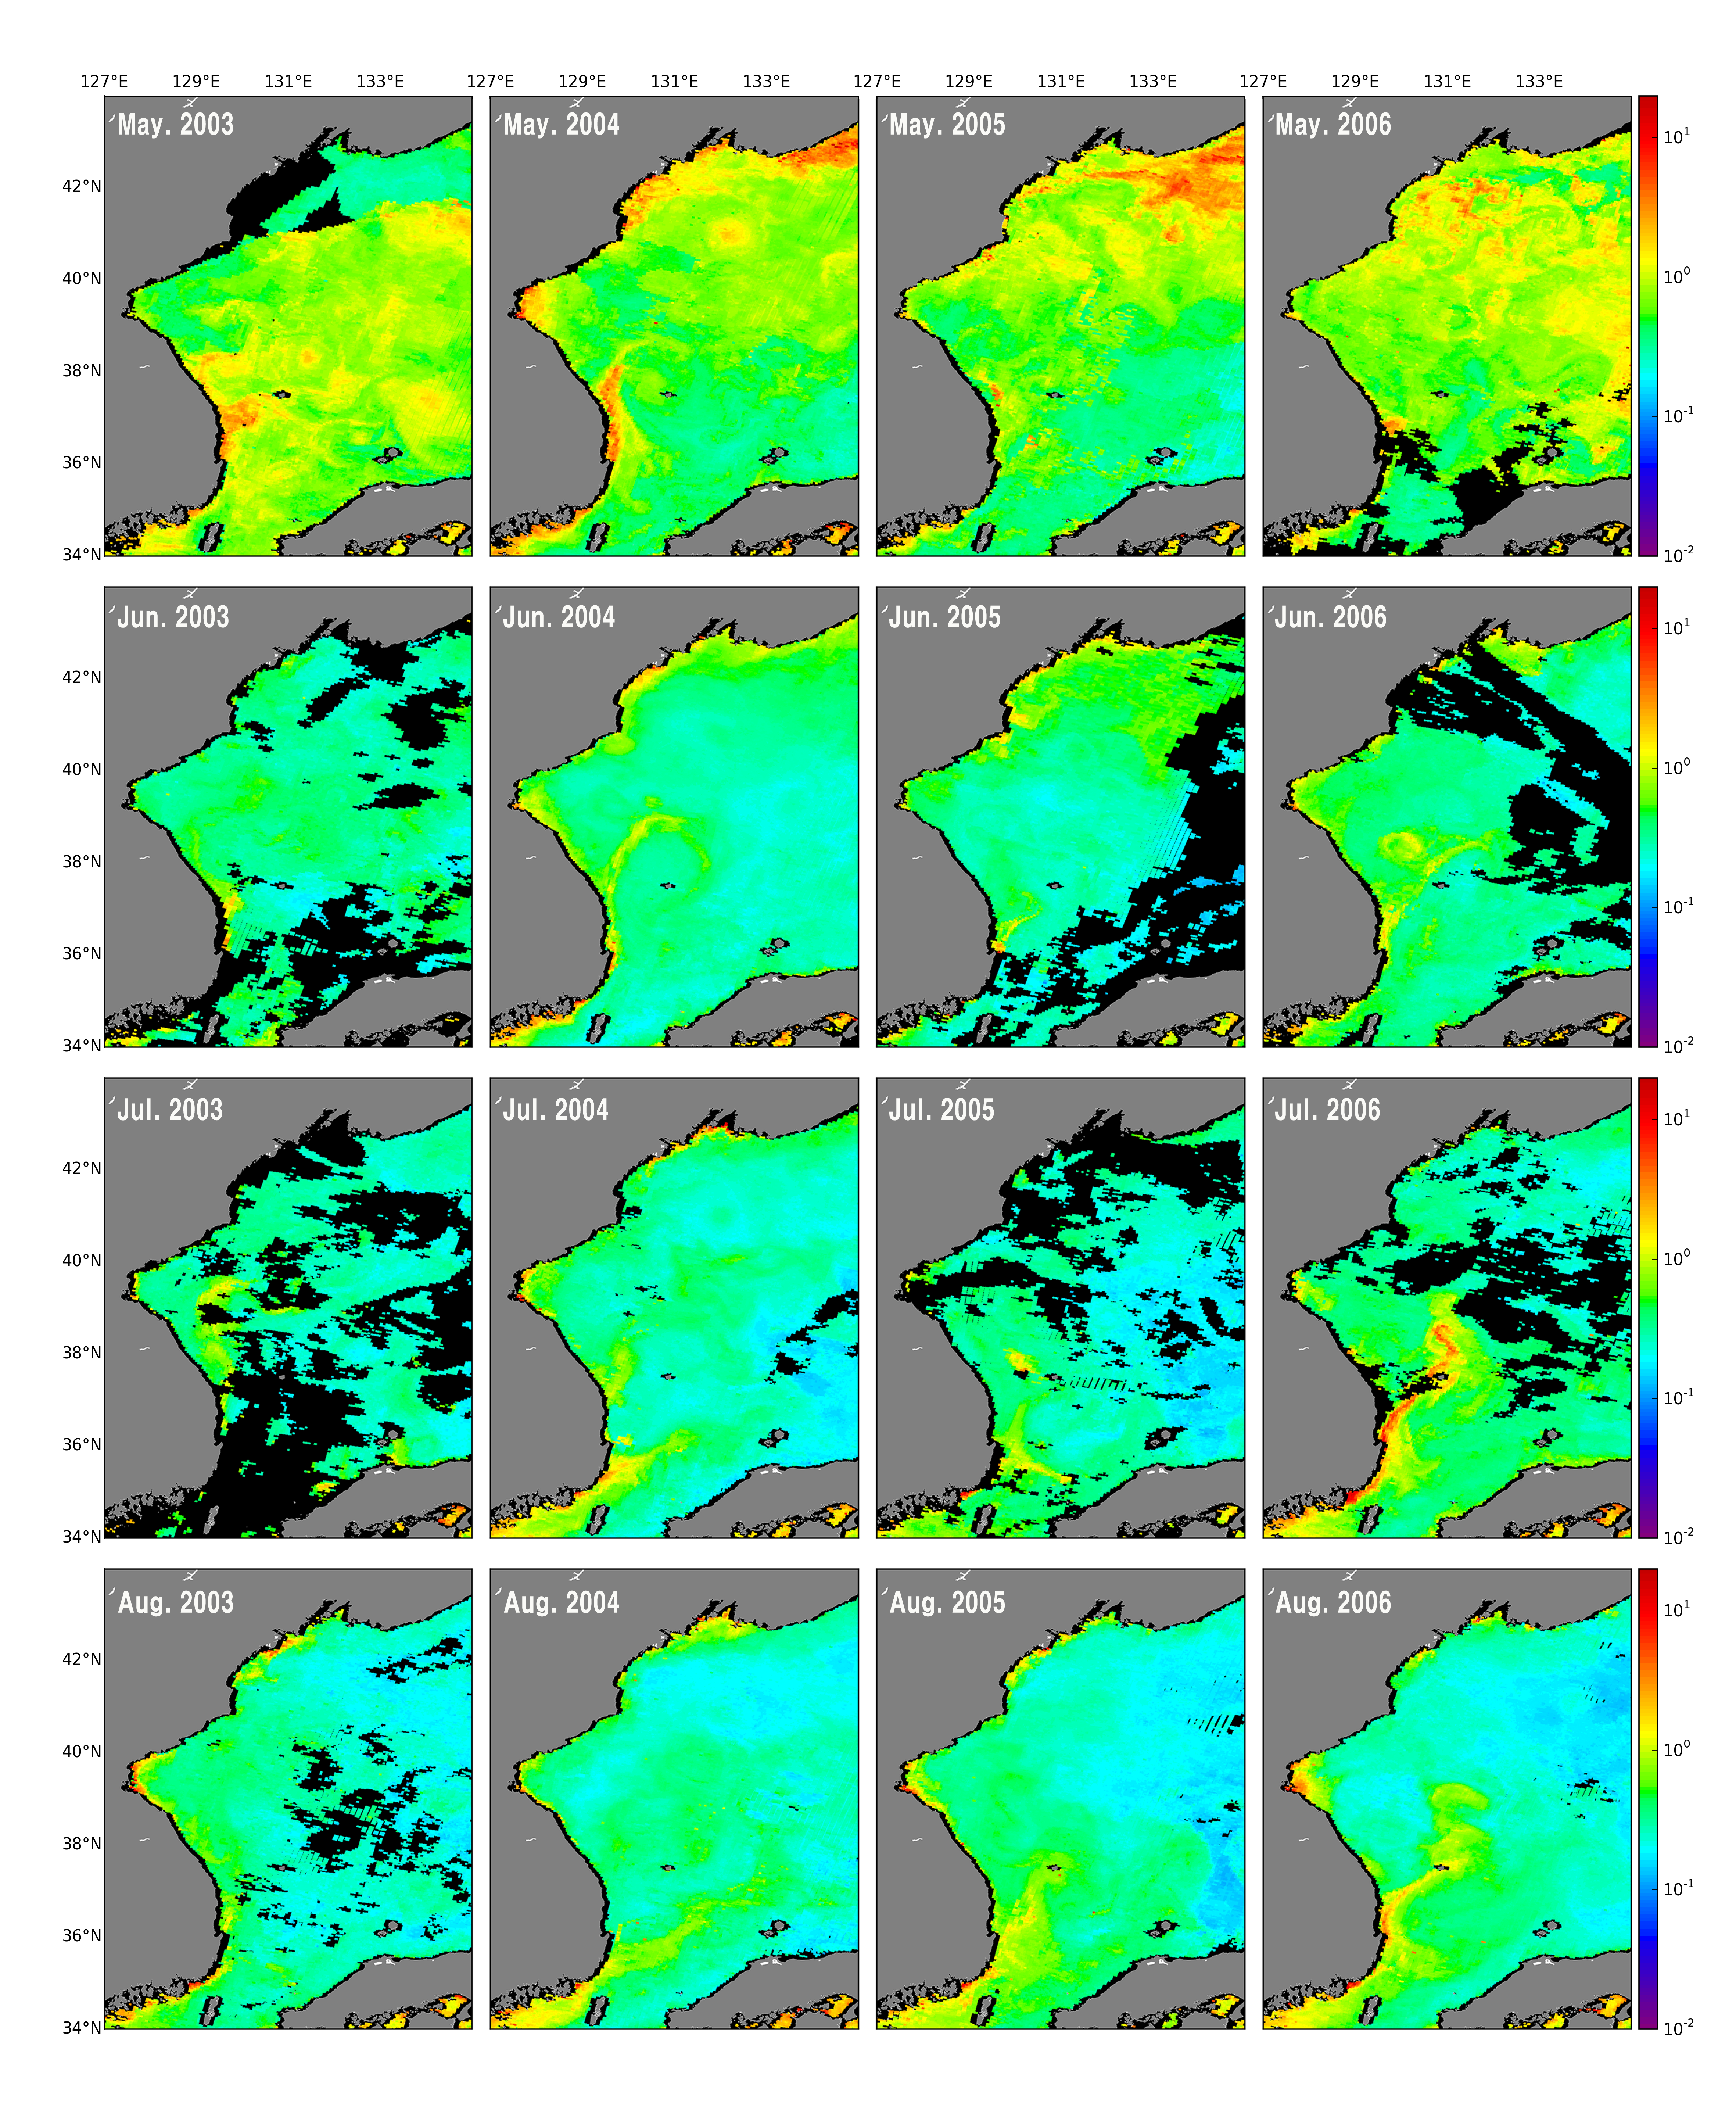
\includegraphics[width=1.00\textwidth]{../images/monGAC02}\\
	\scriptsize\caption{The monthly-mean chlorophyll-a distribution in the East Sea (Sea of Japan), LAC. From 2003 to 2006, May to August. The unit of the color bar is $\rm mg/m^3$.}
	\label{fig:monGAC02}
\end{figure}


\begin{figure}[h]
	\centering
	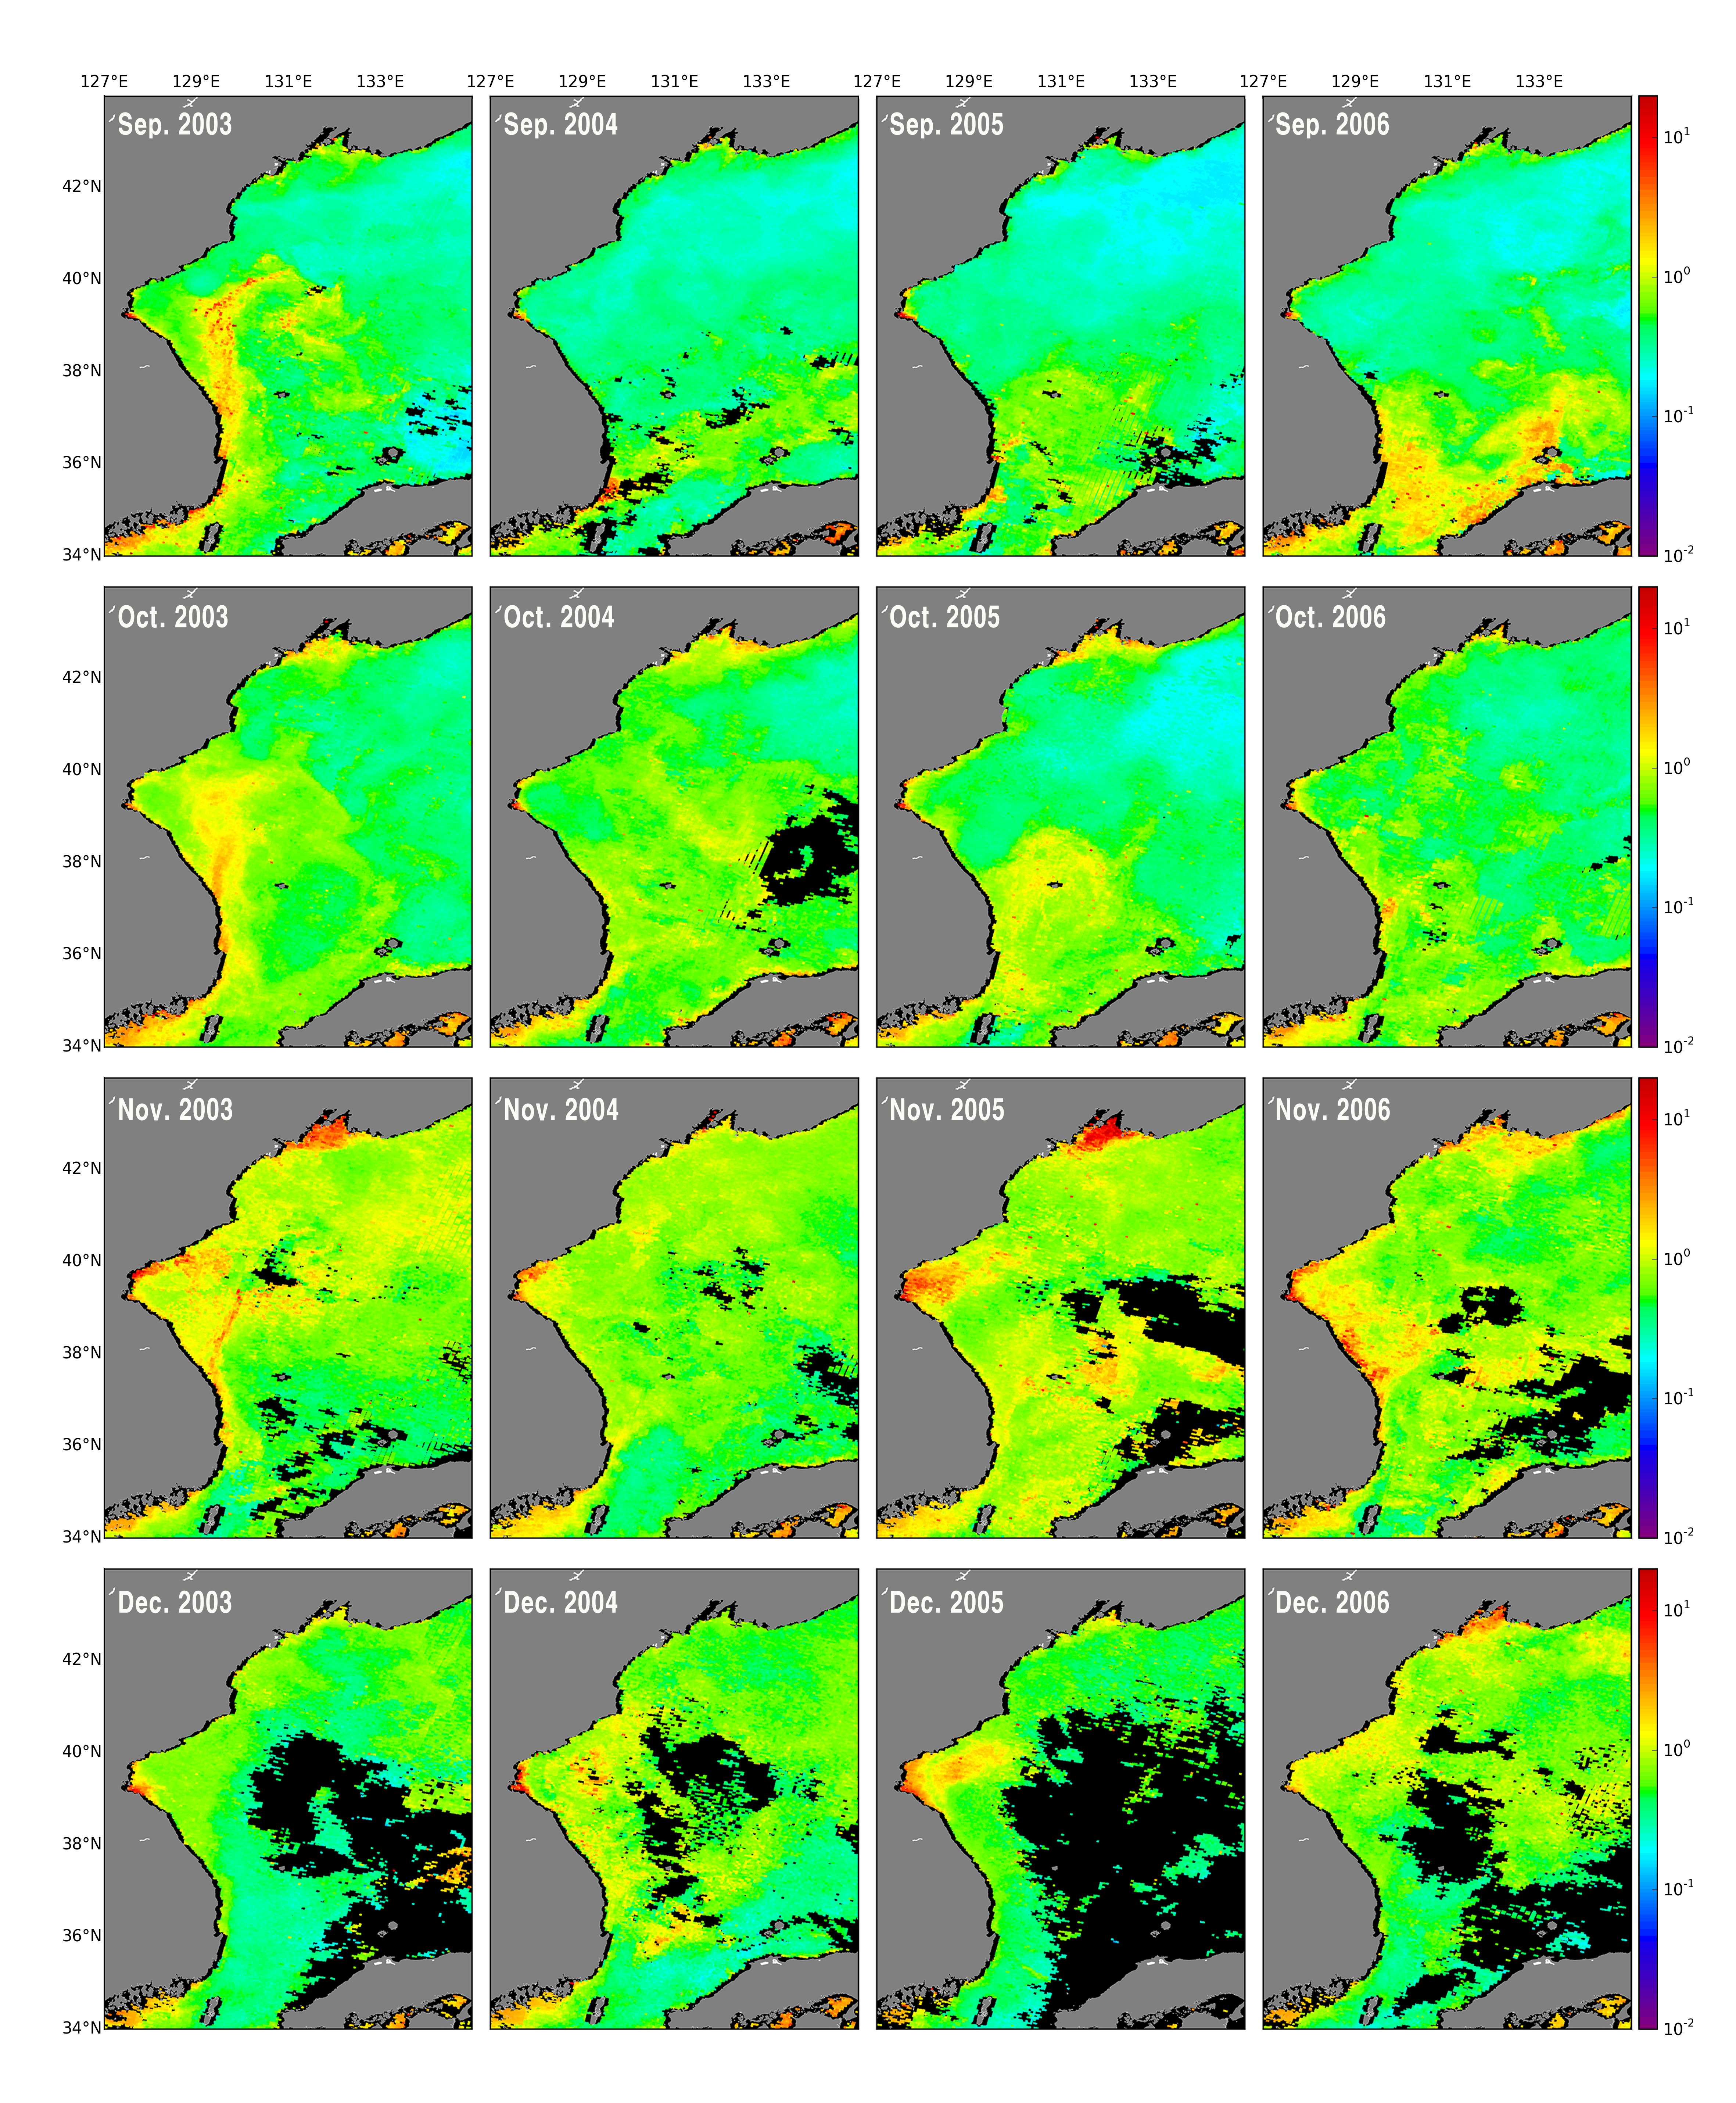
\includegraphics[width=1.00\textwidth]{../images/monGAC03}\\
	\scriptsize\caption{The monthly-mean chlorophyll-a distribution in the East Sea (Sea of Japan), LAC. From 2003 to 2006, September to December. The unit of the color bar is $\rm mg/m^3$.}
	\label{fig:monGAC03}
\end{figure}


